% 译自 arXiv:2306.13589v2 原 tex 第 3951–4189 行（单元 U10）
\section{低维的同调镜像对称}
\thispagestyle{plain}

\takeaway{%
  \textbf{物理图像：}在复维数 1（实维数 2）的最低维情形，同调镜像对称的两侧都能被完全显式地写出来：B-侧是椭圆曲线 $E_\tau=\mathbb{C}/\langle1,\tau\rangle$ 上凝聚层的导出范畴，A-侧是同一个实环面 $\mathbb{T}^2$ 上、以有理斜率测地圈为对象的（富化）Fukaya 范畴。镜像对称在这里退化为「交换复结构参数与复化辛结构参数」。\\
  \textbf{数学工具：}Atiyah 关于椭圆曲线上不可分解向量丛的分类、Jacobi theta 函数、以及 Kreussler 的「校正（rectified）」Fukaya 范畴构造——它以显式的线性代数（局部系统的单值算子、平行移动）取代一般 $A_\infty$ 结构；再加一个预加性范畴到加性范畴的「矩阵化」泛构造。\\
  \textbf{主要结论：}不可分解凝聚层被完全分类（不可分解向量丛，或支撑于一点的不可分解挠层）；$\mathscr{F}^0(E^\rho)$ 只有预加性而无直和，故须经 \underline{$\mathscr{F}^0$} 矩阵化得到 Fukaya--Kontsevich 范畴，才能与 $\mathsf{D^b}(E_\tau)$ 相配。%
}

\subsection{椭圆曲线}\label{ch7.1}


椭圆曲线是同调镜像对称最容易的表现形式。在讨论它之前，本节先考察椭圆曲线的基本特征，包括其导出范畴。主要参考文献为 \cite{[Kre00]} 与 \cite{[Por15]}。

\begin{Def}\label{ellipticcurve}
	\textbf{椭圆曲线}\index{elliptic curve}是指由某个商 $E_\tau\coloneqq\mathbb{C}/\langle 1,\tau\rangle$ 给出的 Riemann 曲面（1 维复流形），其中 $\langle 1,\tau\rangle\coloneqq\mathbb{Z}\oplus\tau\mathbb{Z}\subset\mathbb{C}\cong\mathbb{R}^2$ 是\textbf{模参数}\index{modular parameter} $\tau\in\mathbb{C}$ 所确定的 $\mathbb{Z}^2$-格，并假定 $\mathfrak{Im}(\tau)>0$。其复结构继承自 $\mathbb{C}$。

	此外，商 $\mathbb{C}/\langle 1,\tau\rangle$ 保持 $\mathbb{C}$ 的自然度量与 Kähler 结构：所诱导的 Kähler 形式自动闭，且是最高次微分形式。这使 $E_\tau$ 成为 Kähler 流形，且按定义是紧的。它还可以配上一个全纯体积形式（由紧性，它是 $dz=dx+idy$ 的局部常数倍），满足定义 \ref{Calabiyauman} 的 Calabi--Yau 条件，故 $E_\tau$ 是 1 维 Calabi--Yau 流形。不过要注意：此构造完全忽略了它的辛特征（我们稍后将在定义 \ref{2torus} 中凸显这一点）。

	事实上，可以论证任何 Calabi--Yau 1-维流形必取此形式，即：维数为 1 的一切 Calabi--Yau 流形都是椭圆曲线。
\end{Def}

由第 \ref{ch6.5} 节关于 Calabi--Yau 流形与 Calabi--Yau 簇可否互换的讨论，我们于是关注 1 维光滑射影簇的具体实例，这类对象也称作\textbf{光滑射影曲线}\index{smooth projective curve}。

回想：借助命题 \ref{whenprojvarareequiv}，光滑射影曲线可以被完全分类，唯一的例外正是椭圆曲线：在 \cite[第 5 章]{[Huy06]} 末可见，两条椭圆曲线 $E_{\tau_1}$、$E_{\tau_2}$ 导出等价（即存在正合等价 $\mathsf{D^b}(E_{\tau_1})\rightarrow\mathsf{D^b}(E_{\tau_2})$）当且仅当作为簇有 $E_{\tau_1}\cong E_{\tau_2}$。（这又被用来证明 \cite[推论 5.46]{[Huy06]} 中关于光滑复射影曲线与簇之关系的结果。）

不过，得益于下面这条注，我们无需直接理解椭圆曲线的有界导出范畴。

\begin{Rem}\label{indecomposabletorsion}
	让我们概述两个有用的概念：
	\begin{itemize}[leftmargin=0.5cm]
		\item 设 $(X,\mathcal{O}_X)$ 为任一环空间。则凝聚层 $\mathcal{F}\in\text{obj}(\mathsf{Coh}(X;{}_{\mathcal{O}_X}\!\mathsf{Mod}))$ \textbf{不可分解}\index{ox@$\mathcal{O}_X$-module!indecomposable}，是指它满足
		\[
		\mathcal{F}=\mathcal{F}_1\oplus\mathcal{F}_2\text{ 且 }\mathcal{F}_1,\mathcal{F}_2\in\text{obj}(\mathsf{Coh}(X;{}_{\mathcal{O}_X}\!\mathsf{Mod}))\implies\mathcal{F}_1\cong 0\;\vee\;\mathcal{F}_2\cong 0\,.
		\]
		既然提到，正如定义 \ref{dercatofCY} 之后关于 $\mathsf{D^b}(X)$ 的回顾所述，光滑射影曲线 $X$ 的同调维数 $\text{dim}_h(X)=1$。于是按引理 \ref{whendimhleq1}，任一凝聚层有界复形 $\mathcal{F}^\bullet\in\text{obj}(\mathsf{D^b}(X))$ 都可以写成 $\mathcal{F}^\bullet\cong\bigoplus_{n\in\mathbb{Z}} H^n(\mathcal{F}^\bullet)[-n]^\bullet\in\text{obj}(\mathsf{D^b}(X))$。
		\newline 这就告诉我们：$\mathsf{D^b}(X)$ 中由「诸 $\mathcal{F}[-n]^\bullet\in\text{obj}(\mathsf{D^b}(X))$（其中每个 $\mathcal{F}\in\text{obj}(\mathsf{Coh}(X;{}_{\mathcal{O}_X}\!\mathsf{Mod}))$ 不可分解）的有限直和」构成的有界复形所组成的全子范畴，等价于 $\mathsf{D^b}(X)$。于是我们可以合法地把注意力限制到该子范畴。

		\item 设 $(X,\mathcal{O}_X)$ 为概形。则\textbf{挠层}\index{sheaf!torsion} $\mathcal{F}\in\text{obj}(\mathsf{Sh}(X;{}_{\mathcal{O}_X}\!\mathsf{Mod}))$ 是指这样的 $\mathcal{O}_X$-模：对每个开集 $U\subset X$，$\mathcal{F}(U)$ 是挠阿贝尔群；等价地，在光滑射影曲线 $X$ 上，$\mathcal{F}$ 是挠层当且仅当它在\textit{泛点} $(0)\in\text{Spec}(\mathbb{C}[x])$（即零理想）处的茎 $\mathcal{F}_{(0)}$ 为零。
		\newline 事实上可以证明：任一 $\mathcal{F}\in\text{obj}(\mathsf{Coh}(X;{}_{\mathcal{O}_X}\!\mathsf{Mod}))$ 都分解为 $\mathcal{F}\cong\mathcal{F}/\mathcal{F}_\text{tor}\oplus\mathcal{F}_\text{tor}$，其中 $\mathcal{F}_\text{tor}$ 是它的挠部分，而 $\mathcal{F}/\mathcal{F}_\text{tor}$ 是余下的局部自由部分（也是无挠的）。进一步假定 $\mathcal{F}$ 不可分解，则它或者是一个不可分解的局部自由层（由命题 \ref{locfreeisvectorbundle}，即向量丛），或者是一个支撑在一点上的不可分解挠层（即在仅一个 $x\in X$ 处有 $\mathcal{F}_x\ncong 0$；我们可称 $\mathcal{F}$ 为\textit{加厚摩天楼层}）。
	\end{itemize}
\end{Rem}

% [Tutor Note: 这里的「同调维数 $=1$ 故复形分裂为各阶上同调的平移直和」是一个极易被忽略的关键简化：它把 $\mathsf{D^b}(X)$ 上的问题化归为逐层（逐上同调）的问题，从而只需分类不可分解的**层**，而不必处理复形间的 $\text{Ext}^{\geq 2}$。这也是为什么椭圆曲线的 HMS 能被算出而高维情形不能。另注意「挠层」在光滑曲线上的刻画依赖泛点：$\mathcal{F}_{(0)}=0$ 等价于 $\mathcal{F}$ 的秩为 0，即在开稠密集上为 0。]

为专门弄清椭圆曲线上不可分解凝聚层长什么样，我们先引入一些记号。

\begin{Pro}\label{linebundleonell}
	设 $E_\tau$ 为椭圆曲线。则 $E_\tau$ 上任一线丛都形如
	\begin{equation}
		\mathcal{L}_\tau(\varphi)\coloneqq(\mathbb{C}\oplus\mathbb{C})/\langle1,\tau\rangle\in\textup{obj}(\mathsf{Sh}^\mathsf{lf}_1(E_\tau;{}_{\mathcal{O}_{E_\tau}}\!\mathsf{Mod}))\,,
	\end{equation}
	其中 $\varphi:\mathbb{C}\rightarrow\mathbb{C}^\times$ 是满足「对一切 $z\in\mathbb{C}$ 有 $\varphi(z+1)=\varphi(z)$」的全纯函数，而格 $\langle 1,\tau\rangle$ 通过 $1\cdot(z_1,z_2)=(z_1,z_2)$ 与 $\tau\cdot(z_1,z_2)=(z_1+\tau,\varphi(z_1)z_2)$ 作用。\footnote{由此可知，任一整体截面 $f\in\mathcal{L}_\tau(\varphi)(E_\tau)$ 就是一个全纯函数 $f:\mathbb{C}\rightarrow\mathbb{C}$，使得对一切 $z\in\mathbb{C}$ 有 $f(z+\tau)=\varphi(z)f(z)$ 及 $f(z+1)=f(z)$。} 反过来，任何这样的 $\varphi$ 都可写成
	\[
	\varphi=t_x^*\varphi_0\cdot\varphi_0^{n-1}:\mathbb{C}\rightarrow\mathbb{C}^\times,\,z\mapsto\varphi_0(z+x)\cdot\varphi_0^{n-1}(z)
	\]
	其中 $x=a\tau+b\in E_\tau$、$n\in\mathbb{Z}$，而 $\varphi_0:\mathbb{C}\rightarrow\mathbb{C}^\times,\,z\mapsto e^{-\pi i(\tau+2z)}$。

	此外，整体截面空间 $H^0(\mathcal{L}_\tau(t_x^*\varphi_0^n))$ 是 $n$ 维的，一组可能的基由 $\big(t_x^*\theta[\frac{k}{n},0](n\tau,nz)\big)_{k=0}^{n-1}$ 给出，其中 $\theta$ 表示 \textbf{Jacobi theta 函数}\index{Jacobi theta-function}，定义为
	\begin{equation}
		\theta[a,b](\tau,z)\coloneqq\sum_{n\in\mathbb{Z}}\textup{exp}(\pi i(n+a)^2\tau + 2\pi i(n+a)(z+b))\,.
	\end{equation}
	（它们与经典 theta 函数 $\theta_\tau(z)\coloneqq\sum_{n\in\mathbb{Z}}e^{\pi i(n^2\tau+2nz)}$ 的关系见 \textup{\cite[第 4.1 节]{[Por15]}}，该处还给出 theta 函数之积等有用恒等式。）
\end{Pro}

\begin{Def}\label{unipotentvectorbundle}
	向量丛 $F\rightarrow E_\tau$ 称为\textbf{幂幺的}\index{vector bundle!unipotent}，若在 $\mathsf{Sh}^\mathsf{lf}_1(E_\tau;{}_{\mathcal{O}_{E_\tau}}\!\mathsf{Mod})$ 中存在过滤 $0=F_0\subset F_1\subset...\subset F_r=F$ 使得对所有 $0\leq i< r$ 有 $F_{i+1}/F_i\cong\mathcal{O}_{E_\tau}$。

	给定 $V\in\text{obj}(\mathsf{Vect}_\mathbb{C})$ 与 $A\in\text{GL}(V)$，我们特别地记 $F_\tau(V,A)\!\coloneqq(\mathbb{C}\oplus V)/\langle 1,\tau\rangle$，以表示由作用 $1\cdot(z_1,z_2)=(z_1,z_2)$ 与 $\tau\cdot(z_1,z_2)=(z_1+\tau,Az_2)$ 所决定的那些向量丛。若 $A=e^N$ 而 $N\in\text{End}(V)$ 幂零，则 $F_\tau(V,e^N)$ 是幂幺的；若再有 $\text{dim}(\ker(N))=1$（即 $N$ 是\textit{循环的}），则 $F_\tau(V,e^N)$ 还不可分解。
\end{Def}

我们刚给出的构造看起来有些零散，但出乎意料的是，它们其实正是分类椭圆曲线上不可分解向量丛所需的全部材料——此即 Atiyah 在 \cite{[Ati57]} 中所证。

\begin{Thm}\label{AtiyahThm}
	设 $E_\tau$ 为椭圆曲线。$E_\tau$ 上任一不可分解向量丛都形如 $\pi_{r*}(\mathcal{L}_{r\tau}(\varphi)\otimes F_{r\tau}(V,e^N))$，其中 $N$ 为循环幂零自同态。这里 $\pi_r:E_{r\tau}\rightarrow E_\tau$ 是\textbf{同源}\index{isogeny}——即核有限的满代数群同态——由格包含 $\langle 1,r\tau\rangle\subset\langle 1,\tau\rangle$ 对某个 $r\in\mathbb{R}^+$ 所诱导。
\end{Thm}

% [Tutor Note: Atiyah 的这条分类定理是 1 维情形的核心支柱，其原文（\cite{[Ati57]}）还给出更精细的结论：不可分解向量丛由一对 $(\text{秩},\text{次数})$ 的同余类（$d\equiv 0 \bmod r$）唯一确定，而上述 $\pi_{r*}(\mathcal{L}_{r\tau}(\varphi)\otimes F_{r\tau}(V,e^N))$ 是其显式实现。易错处有二：① 同源 $\pi_r$ 是「$r$ 倍」映射，其像/核的阶与 $r$ 相关，此处 $r\in\mathbb{R}^+$ 而非仅整数，因为同源可以复合；② 「循环幂零」条件 $\text{dim}(\ker N)=1$ 正是保证不可分解性的关键，去掉它只会得到可分解的直和。]

由注 \ref{indecomposabletorsion}，一个不可分解、但并非不可分解向量丛的凝聚层 $\mathcal{E}\in\text{obj}(\mathsf{Coh}(E_\tau;{}_{\mathcal{O}_{E_\tau}}\!\mathsf{Mod})$，必定是支撑于一点 $x\in E_\tau$ 的不可分解挠层；它完全由整体截面空间 $V\coloneqq\mathcal{E}(E_\tau)\in\text{obj}(\mathsf{Vect}_\mathbb{C})$（这同时也是一个 $\mathcal{O}_{E_\tau,x}$-模，其极大理想由 $f(z)=z-x$ 生成）以及某个循环幂零 $N\in\text{End}(V)$ 的选择所决定；此时我们把 $\mathcal{E}$ 写作
\begin{equation}\label{elliptictorsionsheaf}
\mathcal{S}(x,V,N)\coloneqq(\mathcal{O}_{E_\tau,x}\otimes V)/\langle f(z)-N/2\pi i\rangle\in\text{obj}(\mathsf{Coh}(E_\tau;{}_{\mathcal{O}_{E_\tau}}\!\mathsf{Mod}))\,.
\end{equation}

\begin{Cor}\label{indecompocoherentonell}
	设 $E_\tau$ 为椭圆曲线。任一不可分解凝聚层 $\mathcal{E}\in\textup{obj}(\mathsf{Coh}(E_\tau;{}_{\mathcal{O}_{E_\tau}}\!\mathsf{Mod}))$ 或是一个如定理 \ref{AtiyahThm} 中那样形如 $\pi_{r*}(\mathcal{L}_{r\tau}(\varphi)\otimes F_{r\tau}(V,e^N))$ 的不可分解向量丛，或是一个如 \eqref{elliptictorsionsheaf} 中那样形如 $\mathcal{S}(x,V,N)$ 的不可分解挠层；两种情形下 $N\in\textup{End}(V)$ 都是循环幂零的。
\end{Cor}

在转向 A-侧之前，我们提供一条方便的引理，它将在椭圆曲线同调镜像对称的证明中被用到。

\begin{Lem}\label{ellSerreduality}
	设 $E_\tau$ 为椭圆曲线，$\mathcal{E}_1,\mathcal{E}_2\in\textup{obj}(\mathsf{Coh}(E_\tau;{}_{\mathcal{O}_{E_\tau}}\!\mathsf{Mod}))$。则存在函子性同构
	\begin{equation}
		\begin{aligned}
			&\textup{Hom}_{\mathsf{D^b}(E_\tau)}(\mathcal{E}_1[0]^\bullet,\mathcal{E}_2[0]^\bullet)=\textup{Ext}_{\mathcal{O}_{E_\tau}}^0(\mathcal{E}_1,\mathcal{E}_2)\cong\textup{Hom}_{\mathcal{O}_{E_\tau}}(\mathcal{E}_1,\mathcal{E}_2)\,, \\
			&\textup{Hom}_{\mathsf{D^b}(E_\tau)}(\mathcal{E}_1[0]^\bullet,\mathcal{E}_2[1]^\bullet)=\textup{Ext}_{\mathcal{O}_{E_\tau}}^1(\mathcal{E}_1,\mathcal{E}_2)\cong\textup{Hom}_{\mathcal{O}_{E_\tau}}(\mathcal{E}_2,\mathcal{E}_1)^*\,,
		\end{aligned}
	\end{equation}
	而对任何其他 $k\in\mathbb{Z}$ 有 $\textup{Hom}_{\mathsf{D^b}(E_\tau)}(\mathcal{E}_1[0]^\bullet,\mathcal{E}_2[k]^\bullet)=\textup{Ext}_{\mathcal{O}_{E_\tau}}^k(\mathcal{E}_1,\mathcal{E}_2)\cong\{0\}$。

	由此可知，$\diamond:\textup{Ext}_{\mathcal{O}_{E_\tau}}^1(\mathcal{E}_2,\mathcal{E}_3)\times\textup{Ext}_{\mathcal{O}_{E_\tau}}^0(\mathcal{E}_1,\mathcal{E}_2)\rightarrow \textup{Ext}_{\mathcal{O}_{E_\tau}}^1(\mathcal{E}_1,\mathcal{E}_3)$ 与 $\diamond:\textup{Ext}_{\mathcal{O}_{E_\tau}}^0(\mathcal{E}_2,\mathcal{E}_3)\times\textup{Ext}_{\mathcal{O}_{E_\tau}}^1(\mathcal{E}_1,\mathcal{E}_2)\rightarrow \textup{Ext}_{\mathcal{O}_{E_\tau}}^1(\mathcal{E}_1,\mathcal{E}_3)\cong\textup{Hom}_{\mathcal{O}_{E_\tau}}(\mathcal{E}_3,\mathcal{E}_1)^*$ 可以分别解释为映射 $(F,f)\mapsto F(f\circ\square)$ 与 $(f,F)\mapsto F(\square\circ f)$，其中 $f$ 是适当的 \textup{Hom}-态射，而 $F$ 是对偶 \textup{Hom}-空间中的泛函。
\end{Lem}

\begin{proof}（\textit{略证}）
	$k\neq 1$ 的情形按 Ext-模的定义以及 $\text{dim}(E_\tau)=1$（故高阶 Ext 消失）如常得到。对 $k=1$，按 \cite[引理 2.7]{[Kre00]} 的做法细化 Serre 对偶（定理 \ref{Serreduality} 或推论 \ref{SerredualityviaSerrefunc}）的证明即可。
\end{proof}

% [Tutor Note: 这条引理是 1 维情形的「对称性」来源，务必看清其内容：不仅 $\text{Ext}^1(\mathcal{E}_1,\mathcal{E}_2)\cong\text{Hom}(\mathcal{E}_2,\mathcal{E}_1)^*$（这是 Serre 对偶的 $n=1$ 特例），而且 $\text{Ext}^0$ 就是普通 Hom。**正因如此**，在椭圆曲线上 $\text{Ext}$ 代数只在 0、1 两阶非零，且 1 阶通过「对偶 + 反向」与 0 阶相连——这恰是 A-侧「辛 Serre 对偶」\eqref{sympSerreduality} 的 B-侧镜像。作者写「略证」，实际省略的是 Kreussler \cite[引理 2.7]{[Kre00]} 中对 Serre 对偶证明的仿射化改写。]


\subsection{椭圆曲线的 Fukaya 范畴}\label{ch7.2}


现在构造椭圆曲线的 A-侧，并看到它们满足同调镜像对称的一个简化版本；此版本先由 Polishchuk 与 Zaslow 在 \cite{[PZ00]} 中讨论，继而由 Kreussler 在 \cite{[Kre00]} 中更严格地证明。首先，让我们把椭圆曲线的辛结构说得更明确些，即描述猜想 \ref{HMSconj} 所预言的它们的镜像流形。

\begin{Def}\label{2torus}
	设 $\mathbb{T}^2=\mathbb{R}^2/\mathbb{Z}^2$ 为 \textbf{2-环面}\index{2-torus}，它是配以 Kähler 形式 $\kappa\coloneqq Adx\wedge dy\in\Omega^2(\mathbb{T}^2)$ 的 Kähler 流形，其中 $A>0$ 表示其体积（或 Euclid 面积）。在 $H^2_\text{dR}(\mathbb{T}^2;\mathbb{R})/H^2_\text{dR}(\mathbb{T}^2;\mathbb{Z})$ 中选取一个「B-场」，由 $Bdx\wedge dy\in\Omega^2(\mathbb{T}^2)$（某个 $B\in\mathbb{R}$）代表，便定义了\textbf{复化 Kähler 参数}\index{complexified Kähler parameter} $\rho\coloneqq B+iA\in\mathbb{C}$，其中 $\mathfrak{Im}(\rho)>0$；它为 $\mathbb{T}^2$ 提供复化 Kähler 形式 $\rho dx\wedge dy\in\Omega^{1,1}(\mathbb{T}^2)$，并使我们能把该 2-环面解释为模参数为 $\rho$ 的椭圆曲线，从而特别地解释为 1 维 Calabi--Yau 流形。

	我们把配以这样的 $\rho$ 的 $\mathbb{T}^2$ 记为 $E^\rho$。注意：此构造完全忽略了它作为椭圆曲线的复结构。
\end{Def}

由 \cite[定义 6.13]{[Imp21]} 我们知道，刻画 A-侧的 Fukaya 范畴之一般构造是高度非平凡的：对象是（紧、可定向、自旋、分次的）Maslov 类为零的拉格朗日子流形，满足「无泡」条件，并配以分次提升与自旋结构的选择；态射属于构成 Floer 上链复形的分次自由模，其定义依赖于对每元组对象所作的扰动与 Floer 数据的选择；最后还有多线性高阶复合映射，由计数以拉格朗日子流形为边界的伪全纯圆盘得到，它们满足 $A_\infty$-结合性方程。由此得到一个 $A_\infty$-范畴，而为猜想 \ref{HMSconj} 之需，还须考虑其「富化」版本（见 \cite[定义 7.25]{[Imp21]}），其中谈及分裂封闭导出范畴 $\mathscr{F}^0(E^\rho)\coloneqq\mathsf{D}^\pi(\widetilde{\mathscr{F}}(E^\rho))=H^0\big(\Pi(Tw\widetilde{\mathscr{F}}(E^\rho))\big)$。这真是令人生畏的任务！

幸好，在椭圆曲线这一 1 维情形中可作若干简化，使我们的分析轻松许多。例如，\cite[命题 6.31]{[Imp21]} 中略述了 $\mathscr{F}(\mathbb{T}^2)$ 如何可由一对经线与纬线回路分裂生成。然而最省事的策略是：干脆抛开 $E^\rho$ 的富化 Fukaya 范畴的 $A_\infty$-结构，而\textit{直接}定义后者。这么做时我们紧跟 \cite[第 3 节]{[Kre00]} 的「校正（rectified）」版本。

\begin{Def}\label{F0Erho}
	设 $E^\rho$ 为定义 \ref{2torus} 中的 2-环面。则 $\mathscr{F}^0(E^\rho)$ 的对象是三元组 $L=(\Lambda,\alpha, M)\in\text{obj}(\mathscr{F}^0(E^\rho))$，其中：
	\begin{itemize}[leftmargin=0.5cm]
		\renewcommand{\labelitemi}{\textendash}
		\item $\Lambda\subset E^\rho$ 是闭子流形，由 $\mathbb{R}^2$ 中一条有理斜率的仿射直线 $(x(t),y(t))$（$t\in\mathbb{R}$）取商得到，于是我们在 $E^\rho$ 中得到一条\textbf{简单闭曲线}\index{simple loop}（即不自交的闭曲线；参见下文图 \ref{2toruscompo} 或 \cite[例 6.30]{[Imp21]}）。配以定向的选择之后，这样的 $\Lambda$ 恰是 $E^\rho$ 的特殊拉格朗日子流形（它们正是 $E^\rho$ 的全部测地线，反之亦然）。\footnote{关于特殊拉格朗日子流形以及极小、校准子流形等相关概念的简要综述，见 \cite[附录 B]{[Por15]}。}

		\item $\alpha\in\mathbb{R}$ 满足：存在某个 $t_0\in\mathbb{R}$ 使得 $x(0)+iy(0)+e^{i\pi\alpha}=x(t_0)+iy(t_0)$；此即确定了 $\Lambda=(x(t),y(t))$ 的\textbf{分次}\index{grading (of a loop)}（它被用来定义 Maslov 指标）。

		\item $M$ 是 \textit{局部系统}的简写\footnote{等价地，局部系统就是局部常值的复向量空间层，或带有平坦联络的复向量丛（\cite[定义 7.23]{[Imp21]} 所采的变体）。}，该系统由\textbf{单值算子}\index{monodromy operator} $M\in\text{GL}(V)$ 决定，$M$ 的特征值模均为 1：$V$ 是 $r:\pi_1(\Lambda)=\pi_1(\mathbb{S}^1)\cong\mathbb{Z}\rightarrow\text{GL}(V)$ 的表示空间，而 $M$ 是 $\mathbb{Z}$-生成元 $z_M$ 在 $r$ 下的像，$z_M$ 由 $\Lambda$ 上的定向给定，该定向来自 $e^{i\pi\beta}$，其中 $\beta\in(-\frac{1}{2},\frac{1}{2})$ 是使 $\beta-\alpha\in\mathbb{Z}$ 的唯一实数。
	\end{itemize}
	此外，对任一 $L=(\Lambda,\alpha, M)\in\text{obj}(\mathscr{F}^0(E^\rho))$ 与 $x\in \Lambda$，我们固定一个区间 $\{\tilde{x}+t\lambda\mid 0\leq t\leq 1\}\subset\tilde{\Lambda}$，其中 $\tilde{\Lambda}$ 是 $\Lambda$ 的万有覆盖（即 $\mathbb{R}^2$ 中相应的未取商仿射直线），$\lambda\in\mathbb{R}^2$ 是平行于 $\tilde{\Lambda}$、表示 $z_M$ 之提升的唯一向量（在取正向定向下），而 $\tilde{x}\in\tilde{\Lambda}$ 是该区间中映到 $x$ 的适当点，它进而被用来替代 $V\cong M_x$。
\end{Def}

\begin{Def}
	范畴 $\mathscr{F}^0(E^\rho)$ 配以平移函子 $T^1:\mathscr{F}^0(E^\rho)\rightarrow \mathscr{F}^0(E^\rho),\,(\Lambda,\alpha, M)\mapsto (\Lambda,\alpha, M)[1]\coloneqq (\Lambda,\alpha+1, M)$。

	现考虑两个对象 $L_k=(\Lambda_k,\alpha_k, M_k)\in\text{obj}(\mathscr{F}^0(E^\rho))$（$k=0,1$），并令 $\alpha\coloneqq\alpha_1-\alpha_0\in\mathbb{R}$。对其 Hom-空间，我们须区分两种情形：
	\begin{itemize}[leftmargin=0.5cm]
		\renewcommand{\labelitemi}{\textendash}
		\item 若 $\Lambda_0\neq\Lambda_1$，则
		\begin{equation}\label{ellmorphfordifferentlambdas}
			\begin{aligned}
				\mkern-12mu\text{Hom}_{\mathscr{F}^0(E^\rho)}(L_0,L_1)\coloneqq
				\begin{cases}
					\{0\} & \text{若 } \alpha\!\notin\! [0,1)\,, \\
					\mkern-33mu\displaystyle{\bigoplus_{\mkern+40mu x\in\Lambda_0\cap\Lambda_1}}\mkern-24mu\text{Hom}((M_0)_x,(M_1)_x) & \text{否则}\,.
				\end{cases}
			\end{aligned}
		\end{equation}

		\item 若 $\Lambda_0=\Lambda_1$（从而 $\alpha\in\mathbb{Z}$），则
		\begin{small}\begin{align}\label{ellmorphforsamelambdas}
				\mkern-6mu\text{Hom}_{\mathscr{F}^0(E^\rho)}(L_0,L_1)&\coloneqq
				{\begin{cases}
						\{0\} & \text{若 } \alpha\neq 0,1\,, \\
						H^0(\Lambda_0,\mathcal{H}om(M_0,M_1)) & \text{若 } \alpha=0\,, \\
						H^1(\Lambda_0,\mathcal{H}om(M_0,M_1)) & \text{若 } \alpha=1
				\end{cases}} \\
				&\,\cong\begin{cases}
					\{0\} & \text{若 } \alpha\neq 0,1\,, \\
					\{f\!\in\!\text{Hom}(V_0,V_1)\mid M_1\!\circ\! f\!=\!f\!\circ\! M_0\} & \text{若 } \alpha=0\,, \\
					\text{Hom}(V_0,V_1)/M_1\!\circ\!\text{Hom}(V_0,V_1)\!\circ\! M_0^{-1} & \text{若 } \alpha=1\,.
				\end{cases}\nonumber
		\end{align}\end{small}
	\end{itemize}
	特别地，对任意 $L_0,L_1\in\text{obj}(\mathscr{F}^0(E^\rho))$，\textbf{「辛」Serre 对偶}\index{symplectic@``symplectic'' Serre duality}成立：
	\begin{equation}\label{sympSerreduality}
		\text{Hom}_{\mathscr{F}^0(E^\rho)}(L_0,L_1[1])\cong\text{Hom}_{\mathscr{F}^0(E^\rho)}(L_1,L_0)^*\,,
	\end{equation}
	且此同构是典范的、函子性的。
\end{Def}

% [Tutor Note: 此处原文用 `$if $`、`$else$` 之类的伪 LaTeX 写在 cases 环境中（既非数学也非规范排版），译文按其语义改排为 \text{若}/\text{否则}，公式内容未动。三个易错点：① 第一种情形的 Hom 只在 $\alpha\in[0,1)$ 时非零，即「两张膜之间的**相对分次**落在基本区间内」才可能有态射，这是 Floer 理论的度数约束；② 第二种情形中 $\alpha=0$ 给的是 $M_k$ 的**交换子**空间，$\alpha=1$ 给的是商 $V_0\to V_1$ 模去 $M_1(\cdot)M_0^{-1}$ 的作用——这两式正是「圆柱上的 Floer 上同调即局部系统系数的上同调」的显式化；③ \eqref{sympSerreduality} 与 B-侧的 \ref{ellSerreduality} 必须逐项对照：A-侧的「$[1]$ 平移 ↔ 取对偶」正是 B-侧 $\text{Ext}^1\cong\text{Hom}(\cdot,\cdot)^*$ 的镜像。]

剩下只需定义态射的复合律。由于 \cite{[PZ00]} 只处理了三个两两不同的拉格朗日子流形的情形，我们继续沿用 \cite{[Kre00]} 的细致分析。

\begin{Def}
	设 $L_k=(\Lambda_k,\alpha_k,M_k)\in\text{obj}(\mathscr{F}^0(E^\rho))$（$k=0,1,2$），$u\in\text{Hom}_{\mathscr{F}^0(E^\rho)}(L_0,L_1)$、$v\in\text{Hom}_{\mathscr{F}^0(E^\rho)}(L_1,L_2)$（二者均非零），从而按定义必须有 $\alpha_0\leq\alpha_1\leq \alpha_0+1$ 与 $\alpha_1\leq\alpha_2\leq \alpha_1+1$。为定义 $v\circ u\in\text{Hom}_{\mathscr{F}^0(E^\rho)}(L_0,L_2)$，也即复合律
	\[
	\circ:\text{Hom}_{\mathscr{F}^0(E^\rho)}(L_1,L_2)\otimes\text{Hom}_{\mathscr{F}^0(E^\rho)}(L_0,L_1)\rightarrow \text{Hom}_{\mathscr{F}^0(E^\rho)}(L_0,L_2)\,,
	\]
	我们区分如下情形。
	\begin{itemize}[leftmargin=0.5cm]
		\renewcommand{\labelitemi}{\textendash}
		\item 若 $\alpha_0<\alpha_1<\alpha_2 < \alpha_0+1$，即诸 $L_k$ 两两不同，则给定 $u_{x_0}\in\text{Hom}_{\mathscr{F}^0(E^\rho)}((M_0)_{x_0},(M_1)_{x_0})\subset\text{Hom}_{\mathscr{F}^0(E^\rho)}(L_0,L_1)$（$x_0\in\Lambda_0\cap\Lambda_1$）与 $v_{x_1}\in\text{Hom}_{\mathscr{F}^0(E^\rho)}((M_1)_{x_1},(M_2)_{x_1})\subset\text{Hom}_{\mathscr{F}^0(E^\rho)}(L_1,L_2)$（$x_1\in\Lambda_1\cap\Lambda_2$），我们逐纤维地定义 $v\circ u$ 为
		\begin{equation}
			(v\circ u)_{x_2}\coloneqq\mkern-18mu\sum_{[(\phi;z_0,z_1,z_2)]}\mkern-18mu e^{2\pi i\!\int\!\phi^*(\rho dx\wedge dy)}\mathbb{P}(M_2)\circ v_{x_1}\circ\mathbb{P}(M_1)\circ u_{x_0}\circ\mathbb{P}(M_0)
		\end{equation}
		其取值在 $\text{Hom}_{\mathscr{F}^0(E^\rho)}((M_0)_{x_2},(M_2)_{x_2})$ 中，对任一 $x_2\in \Lambda_0\cap\Lambda_2$。这里 $\mathbb{P}(M_k):(M_k)_{x_{k-1}}$ $\rightarrow (M_k)_{x_k}$ 表示平行移动；而求和\footnote{此过程类似于定义 Floer 积的伪全纯三角形计数，见 \cite[第 6.1 节]{[Imp21]}。}取遍从单位圆盘出发、带互异边界标记点 $z_0,z_1,z_2\in\mathbb{D}^2$ 的全纯映射 $\phi:\mathbb{D}^2\rightarrow E^\rho$ 的所有等价类，满足 $\phi(z_k)=x_k$，且边界弧段 $z_k\!\curvearrowright\! z_{k+1}$ 被映入 $\Lambda_k$（从而 $z_2\!\curvearrowright\! z_0$ 映入 $\Lambda_2$）；两个构型若相差 $\mathbb{D}^2$ 的一个自同构，则视为等价。该情形描绘于下文图 \ref{2toruscompo}。

		\item 若 $\alpha_2>\alpha_0+1$，则 $v\circ u\coloneqq 0$。

		\item 若 $\alpha_0=\alpha_1<\alpha_2$（从而 $\Lambda_0=\Lambda_1\neq\Lambda_2$），则由 \eqref{ellmorphfordifferentlambdas} 的提示，取遍所有 $x\in\Lambda_0\cap\Lambda_2$ 的直和之后，$v\circ u$ 由 $v_x\otimes u\mapsto v_x\circ u_x$ 诱导。$\alpha_0+1=\alpha_1=\alpha_2$ 且 $\Lambda_0\neq\Lambda_1=\Lambda_2$ 的情形同理。

		\item 若 $\alpha_0=\alpha_1=\alpha_2$，从而 $\Lambda_0=\Lambda_1=\Lambda_2$，我们只需复合由 \eqref{ellmorphforsamelambdas} 第二种情形给出的线性同态 $f_k$。

		\item 最后，若 $\alpha_0+1=\alpha_2$，可用辛 Serre 对偶退回到上述某一情形。
	\end{itemize}
	注意：第一个情形其实是唯一依赖于 $\rho$ 的情形。	
\end{Def}

\begin{figure}[htp]
\centering
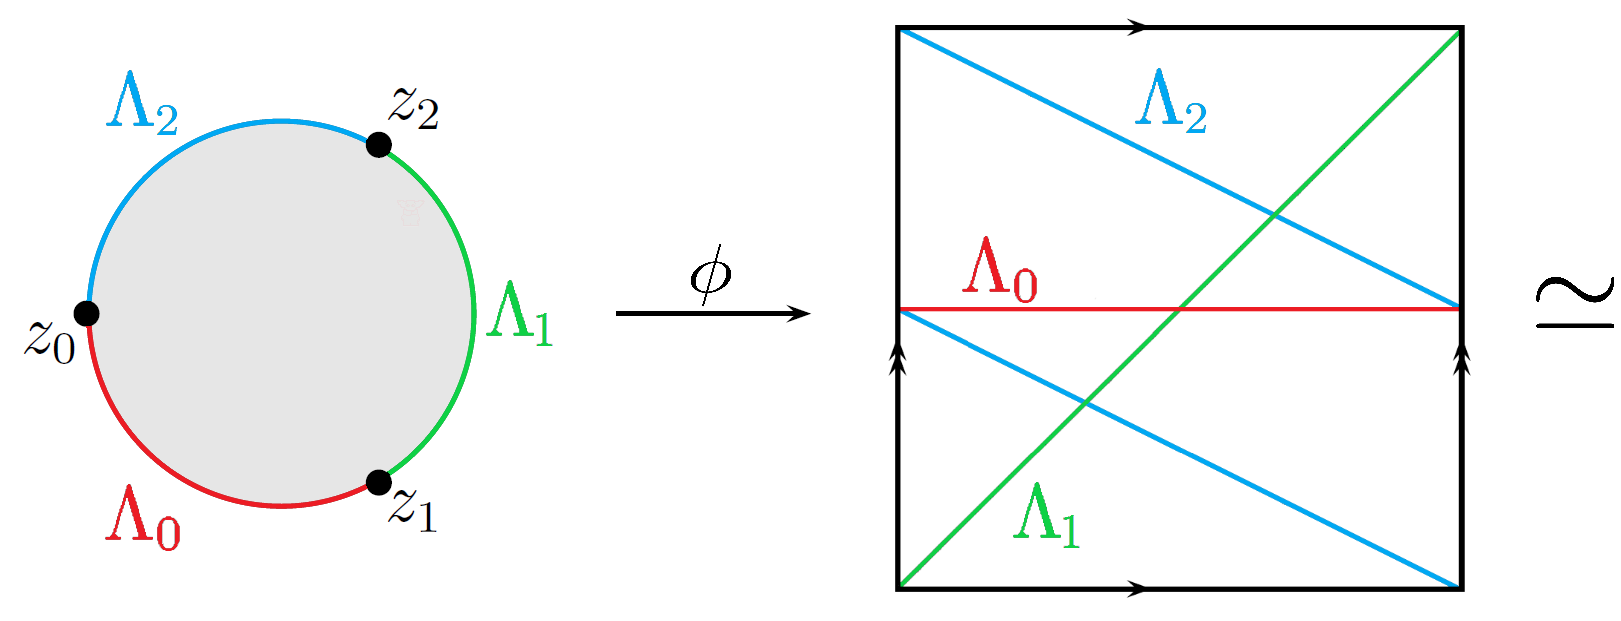
\includegraphics[width=0.6\textwidth]{2toruscompo.png}\quad
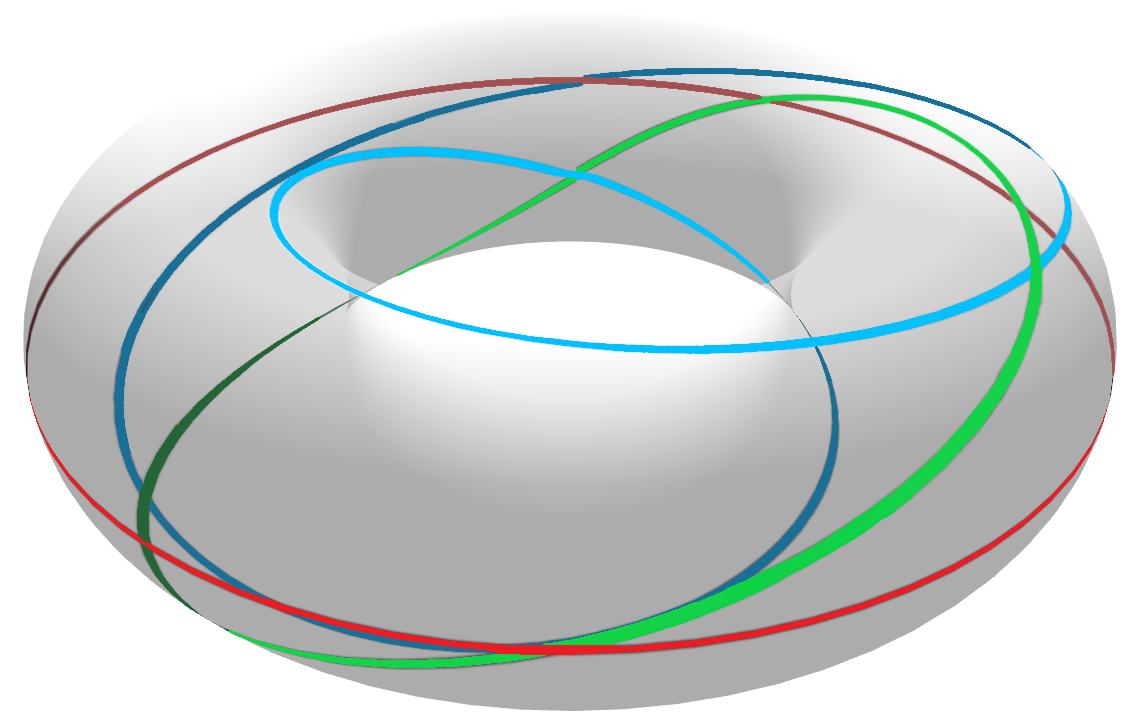
\includegraphics[width=0.35\textwidth]{2torus.png}	
\caption{当拉格朗日子流形彼此不同时，定义复合律所用到的一个可能的映射 $\phi:\mathbb{D}^2\rightarrow E^\rho$。图中特别绘出了 $\mathbb{R}^2$ 模 $\mathbb{Z}^2$ 下的仿射直线 $(t,1/2)$、$(t,t)$ 与 $(t,-t/2+1/2)$，它们分别给出 $\Lambda_0$、$\Lambda_1$ 与 $\Lambda_2$。（原图位置：原 PDF 第 134 页）}
\label{2toruscompo}	
\end{figure}
\vspace*{0.3cm}

% [Tutor Note: 这是全书唯一需要「数圆盘」的地方，也是 $A_\infty$ 范畴的一般定义在此维数下的唯一痕迹。要点：$e^{2\pi i\int\phi^*(\rho dx\wedge dy)}$ 是面积权重——它正是同调镜像对称中把**辛面积** $A$ 与 **B-场** $B$ 合成为复化参数 $\rho=B+iA$ 的物理根源（面积项的相位来自 $B$，模长来自 $A$）。注意 $\phi$ 的边界弧段按**逆时针**依次落入 $\Lambda_0,\Lambda_1,\Lambda_2$，作者用 $z_k\curvearrowright z_{k+1}$ 表示该走向；若把定向约定反过来，则图 \ref{2toruscompo} 中的三角形会取共轭，导致复合律中指数项的符号翻转。]

\noindent 现在我们遇到 \cite{[PZ00]} 最初忽略的主要问题：范畴 $\mathscr{F}^0(E^\rho)$ 是预加性范畴（仅满足定义 \ref{addcat} 的公理 (A1)），却不像一切导出范畴那样是加性范畴（参引理 \ref{D(A)additive}），因为它不含直和，从而不可能构造出同调镜像对称所猜想的任何等价。不过我们注意到下述一般事实。

\begin{Lem}\label{frompreaddtoaddcat}
	设 $\mathsf{C}$ 为预加性范畴，$\underline{\mathsf{C}}$ 为具有如下结构的范畴：
	\begin{itemize}[leftmargin=0.5cm]
		\renewcommand{\labelitemi}{\textendash}

		\item $\textup{obj}(\underline{\mathsf{C}})=\coprod_{k\geq 0}\prod_{l=1}^k\textup{obj}(\mathsf{C})$，于是 $\underline{\mathsf{C}}$ 的对象是 $\mathsf{C}$ 的对象构成的任意长度的有序元组。

		\item 给定 $\underline{X}=(X_1,...,X_k)$ 与 $\underline{Y}=(Y_1,...,Y_l)$（均在 $\textup{obj}(\underline{\mathsf{C}})$ 中，$k,l>0$），令 $\textup{Hom}_{\underline{\mathsf{C}}}(\underline{X},\underline{Y})\coloneqq\prod_{\begin{tiny}1\leq i\leq k, 1\leq j\leq l\end{tiny}}\textup{Hom}_\mathsf{C}(X_i,Y_j)$。随后通过要求零对象 $\underline{0}\in\textup{obj}(\underline{\mathsf{C}})$ 兼具始与终来定义它，即 $\textup{Hom}_{\underline{\mathsf{C}}}(\underline{0},\underline{Y})\coloneqq\{0\}$ 且 $\textup{Hom}_{\underline{\mathsf{C}}}(\underline{X},\underline{0})\coloneqq\{0\}$（若 $\mathsf{C}$ 有零对象 $0_\mathsf{C}$，则任一元组 $(0_\mathsf{C},...,0_\mathsf{C})$ 都同构于 $\underline{0}$）。

		\item 态射的复合律由标准的矩阵乘法给出。
	\end{itemize}
	则 $\underline{\mathsf{C}}$ 是加性范畴，且加性函子 $\mathsf{C}\rightarrow\underline{\mathsf{C}}$（在对象上作用为 $X\mapsto \underline{X}\coloneqq(X)$，即 1-元组）是泛函子（关于「泛」的定义见 \cite[第 III.1 节]{[Har77]}）。
\end{Lem}

这促使我们转而研究由 $\mathscr{F}^0(E^\rho)$ 以此方式诱导的加性范畴，而非 $\mathscr{F}^0(E^\rho)$ 本身。同时，我们开始把模参数 $\rho$ 改记为 $\tau$，以便与将要陈述的同调镜像对称相符。

\begin{Def}\label{FukayaKontsevichcat}
	设 $E^\tau$ 为 2-环面，其分裂封闭导出范畴为 $\mathscr{F}^0(E^\tau)$ $=\mathsf{D}^\pi(\widetilde{\mathscr{F}}(E^\tau))=H^0\big(\Pi(Tw\widetilde{\mathscr{F}}(E^\tau))\big)$。则我们称
	\[
	\mathscr{F\!K}^0(E^\tau)\coloneqq\underline{\mathscr{F}^0(E^\tau)}
	\]
	为 \textbf{Fukaya--Kontsevich 范畴}\index{Fukaya--Kontsevich category}。由引理 \ref{frompreaddtoaddcat} 它是加性范畴，而加性函子 $\mathscr{F}^0(E^\tau)\rightarrow\mathscr{F\!K}^0(E^\tau),\,L\mapsto \underline{L}\coloneqq(L)$ 使我们得以继续在不写下划线的情况下记它的对象与态射。

	对任一 $r\in\mathbb{N}$，令 $p_r:E^{r\tau}\rightarrow E^\tau,\,(x,y)\mapsto(rx,y)$。然后我们定义如下加性函子：
	\begin{itemize}[leftmargin=0.5cm]
		\item $p_{r*}:\mathscr{F\!K}^0(E^{r\tau})\rightarrow \mathscr{F\!K}^0(E^\tau)$，由 $p_{r*}(\Lambda,\alpha,M)\coloneqq (p_r(\Lambda),\alpha',p_{r*}M)$ 给出，其中：$\alpha'\in(k-\frac{1}{2},k+\frac{1}{2}]$ 是满足定义 \ref{F0Erho} 的分次条件的唯一可取之值，而 $k\in\mathbb{Z}$ 由 $\alpha$ 决定（$\alpha$ 必属同一区间）；$p_{r*}M\in\text{GL}(V^{\oplus d})$ 由 $(p_{r*}M)(v_1,...,v_d)\coloneqq(v_2,...,v_d,M(v_1))$ 给出（这里设 $p_r$ 在 $\Lambda$ 上的度数为 $d$）。
		\newline 对任一 $\text{Hom}_{\mathscr{F\!K}^0(E^{r\tau})}(L_0,L_1)$ 中的态射，我们须再次区分 $p_r(\Lambda_0)\neq p_r(\Lambda_1)$、$\Lambda_0=\Lambda_1$ 以及 $\Lambda_0\neq\Lambda_1\,\wedge\,p_r(\Lambda_0)= p_r(\Lambda_1)$ 三种情形，并验证相容性。

		\item $p_r^*:\mathscr{F\!K}^0(E^\tau)\rightarrow\mathscr{F\!K}^0(E^{r\tau})$，取 $p_r^*(\Lambda,\alpha,M)\!\coloneqq\!\bigoplus_{k=1}^n (\Lambda^{(k)},\alpha',(p_r^{(k)})^*M)$，其中：设 $p_r^{-1}(\Lambda)$ 有 $n$ 个连通分支 $\Lambda^{(k)}$，且每个限制 $p_r^{(k)}:\Lambda^{(k)}\rightarrow\Lambda$ 的度数为 $d\coloneqq r/n$；$\alpha'\in(k-\frac{1}{2},k+\frac{1}{2}]$ 仍与 $\alpha$ 同区间；$(p_r^{(k)})^*M=M^d\in\text{GL}(V)$。\footnote{在把局部系统解释为局部常值复向量空间层时，$p_{r*}M$ 表示「给出 $M$ 的那个局部系统之推前」的单值，而 $(p_r^{(k)})^*M$ 表示拉回的单值。} 也正是在这里，「对直和封闭」的必要性显现出来：若 $n>1$，$p_r^*$ 的像并不落在 $\mathscr{F}^0(E^\tau)$ 之中！
		\newline 对态射，我们只需考察拉格朗日子流形相等与不相等两种情形。
	\end{itemize}
\end{Def}

% [Tutor Note: 本节的逻辑主线务必把握：$\mathscr{F}^0$ 只有预加性（Hom-空间是向量空间，但无直和），因此**不可能**与 $\mathsf{D^b}(E_\tau)$（加性）等价——这就是 \cite{[PZ00]} 的漏洞，也是 Kreussler 的贡献所在。引理 \ref{frompreaddtoaddcat} 的「矩阵化」构造 $\underline{\mathsf{C}}$ 是标准的成加性包络（additive envelope）：对象取有限元组、态射取矩阵、复合取矩阵乘法。这样得到的 $\mathscr{F\!K}^0$ 才是可作等价的。另注意 $p_r$ 的推前/拉回在「$n>1$」时确实会跑出原范畴——这正是作者强调「对直和封闭」之处。]
